\documentclass{article}

% Language setting
% Replace `english' with e.g. `spanish' to change the document language
\usepackage[polish]{babel}

% Set page size and margins
% Replace `letterpaper' with`a4paper' for UK/EU standard size
\usepackage[letterpaper,top=2cm,bottom=2cm,left=3cm,right=3cm,marginparwidth=1.75cm]{geometry}

% Useful packages
\usepackage{amsmath}
\usepackage{graphicx}
\usepackage[T1]{fontenc}
\usepackage[noend]{algpseudocode}
\usepackage[linesnumbered,ruled,vlined]{algorithm2e}

%\usepackage[colorlinks=true, allcolors=blue]{hyperref}

\usepackage{hyperref}
\usepackage{tikz}
\usepackage{float}
\usepackage{graphicx}
\usepackage{subcaption}
\usepackage{float}
\usepackage{tabularx}
\usepackage{booktabs}
\usepackage{adjustbox}
\usepackage{multirow}
\usetikzlibrary{shapes,arrows,positioning,calc}

\title{ZUM - dokumentacja końcowa}
\author{Anna Schäfer, Mikołaj Szawerda}

\begin{document}
\maketitle

\section{Zadanie klasyfikacji spamu}

Celem niniejszego sprawozdania jest kompleksowa ocena procesu budowy klasyfikatora wykrywającego wiadomości spam. Badania podzielono na trzy spójne etapy. Najpierw zbadano, w jaki sposób różne warianty wstępnej obróbki tekstu (m.in. usuwanie znaków interpunkcyjnych, liczb, „stop-words” oraz stemming) i pięć metod wektoryzacji (BoW, TF-IDF w wariantach uni- i bigram, oraz dwa rozmiary Word2Vec) wpływają na skuteczność losowego lasu-bazowego klasyfikatora.

W drugiej części porównano pięć algorytmów uczenia (Multinomial NB, liniowy i nieliniowy SVM, Random Forest oraz XGBoost), uwzględniając ich najlepsze zestawy hiperparametrów, wydajność obliczeniową i odporność na trudne przypadki „hard ham”.

Ostatni moduł pracy poświęcono redukcji wymiarowości – od PCA i SVD po wybór cech ANOVA F – dla liniowego SVM trenowanego na macierzy TF-IDF bigram; analizowano wpływ liczby składowych/cech na jakość, czas treningu i zużycie pamięci. 

Implementacja projektu znajduje się w: \href{https://github.com/MikolajSzawerda/25L-zum}{MikolajSzawerda/25L-zum}

\section{Wstępna obróbka danych tekstowych i reprezentacja}

W ramach tej serii eksperymentów sprawdzony został wpływ operacji na danych wejściowych na końcową jakość modelu jak i ich reprezentacji. Modelem testowym w czasie eksperymentów był:

\texttt{RandomForestClassifier(n\_estimators=100, random\_state=42)}.


Sprawdzane operacje:
\begin{itemize}
    \item zmiana na małe litery (\textit{lowercase})
    \item usunięcie interpunkcji (\textit{remove\_punctuation})
    \item usunięcie liczb (\textit{remove\_numbers})
    \item usunięcie "stop words" (\textit{remove\_stopwords}) -- słów o małym znaczeniu semantycznym
    \item usunięcie końcówek fleksyjnych (\textit{stemming})
\end{itemize}

\subsection{Konfiguracja eksperymentów}

\subsubsection{Wstępna obróbka}

Każdy z eksperymentów uruchomiony był z użyciem \texttt{RepeatedStratifiedKFold(n\_splits=5, n\_repeats=3, random\_state=42)} w ramach walidacji krzyżowej.


\begin{table}[h!]
\centering
\begin{tabular}{|l|c|c|c|c|c|c|}
\hline
\textbf{} & \textbf{lowercase} & \textbf{punctuation} & \textbf{numbers} & \textbf{stopwords} & \textbf{stemming} & \textbf{min\_word\_length} \\
\hline
minimal     & True  & False & False & False & False & nan \\
standard    & True  & True  & True  & True  & False & nan \\
aggressive  & True  & True  & True  & True  & True  & nan \\
custom      & True  & True  & False & True  & True  & 3   \\
\hline
\end{tabular}
\caption{Konfiguracje operacji przetwarzania tekstu w poszczególnych eksperymentach}
\end{table}

{\scriptsize
\begin{verbatim}
df['mail'].tolist()
Return-Path: <exmh-workers-admin@spamassassin.taint.org>
Delivered-To: yyyy@localhost.netnoteinc.com
Received:

TextPreprocessor(**PREPROCESSING_CONFIGS['minimal']).transform(df['mail'])
return-path: <exmh-workers-admin@spamassassin.taint.org> delivered-to: yyyy@localhost.netnoteinc.com received:

TextPreprocessor(**PREPROCESSING_CONFIGS['standard']).transform(df['mail'])
return path exmh workers admin spamassassin taint org delivered yyyy localhost netnoteinc com received 

TextPreprocessor(**PREPROCESSING_CONFIGS['aggressive']).transform(df['mail'])
return path exmh worker admin spamassassin taint org deliv yyyi localhost netnoteinc com receiv

TextPreprocessor(**PREPROCESSING_CONFIGS['custom']).transform(df['mail'])
return path exmh worker admin spamassassin taint org deliv yyyi localhost netnoteinc com receiv
\end{verbatim}
}

\subsubsection{Wektoryzacja}
W ramach reprezentacji zbadane zostały(w wersjach unigram i bigram):

\begin{itemize}
    \item BOW
    \item TF-IDF
\end{itemize}

oraz \texttt{Word2Vec}

\begin{table}[h!]
\centering
\begin{adjustbox}{width=\textwidth}
\begin{tabularx}{\textwidth}{|l|X|X|}
\hline
\textbf{} & \textbf{vectorizer} & \textbf{params} \\
\hline
tfidf\_unigram & \texttt{<TfidfVectorizer'>} & \texttt{\{'max\_features': 10000, 'ngram\_range': (1, 1), 'min\_df': 2, 'max\_df': 0.95\}} \\
\hline
tfidf\_bigram & \texttt{<TfidfVectorizer'>} & \texttt{\{'max\_features': 10000, 'ngram\_range': (1, 2), 'min\_df': 2, 'max\_df': 0.95\}} \\
\hline
count\_unigram & \texttt{<CountVectorizer'>} & \texttt{\{'max\_features': 10000, 'ngram\_range': (1, 1), 'min\_df': 2, 'max\_df': 0.95\}} \\
\hline
count\_bigram & \texttt{<.CountVectorizer'>} & \texttt{\{'max\_features': 10000, 'ngram\_range': (1, 2), 'min\_df': 2, 'max\_df': 0.95\}} \\
\hline
word2vec\_skipgram & \texttt{<Word2VecVectorizer'>} & \texttt{\{'vector\_size': 100, 'window': 5, 'min\_count': 1, 'sg': 1, 'epochs': 15, 'seed': 42\}} \\
\hline
word2vec\_large & \texttt{<Word2VecVectorizer'>} & \texttt{\{'vector\_size': 200, 'window': 10, 'min\_count': 2, 'sg': 0, 'epochs': 15, 'seed': 42\}} \\
\hline
\end{tabularx}
\end{adjustbox}
\caption{Konfiguracje wektoryzatorów i ich parametrów}
\end{table}

\begin{figure}[H]
    \centering
    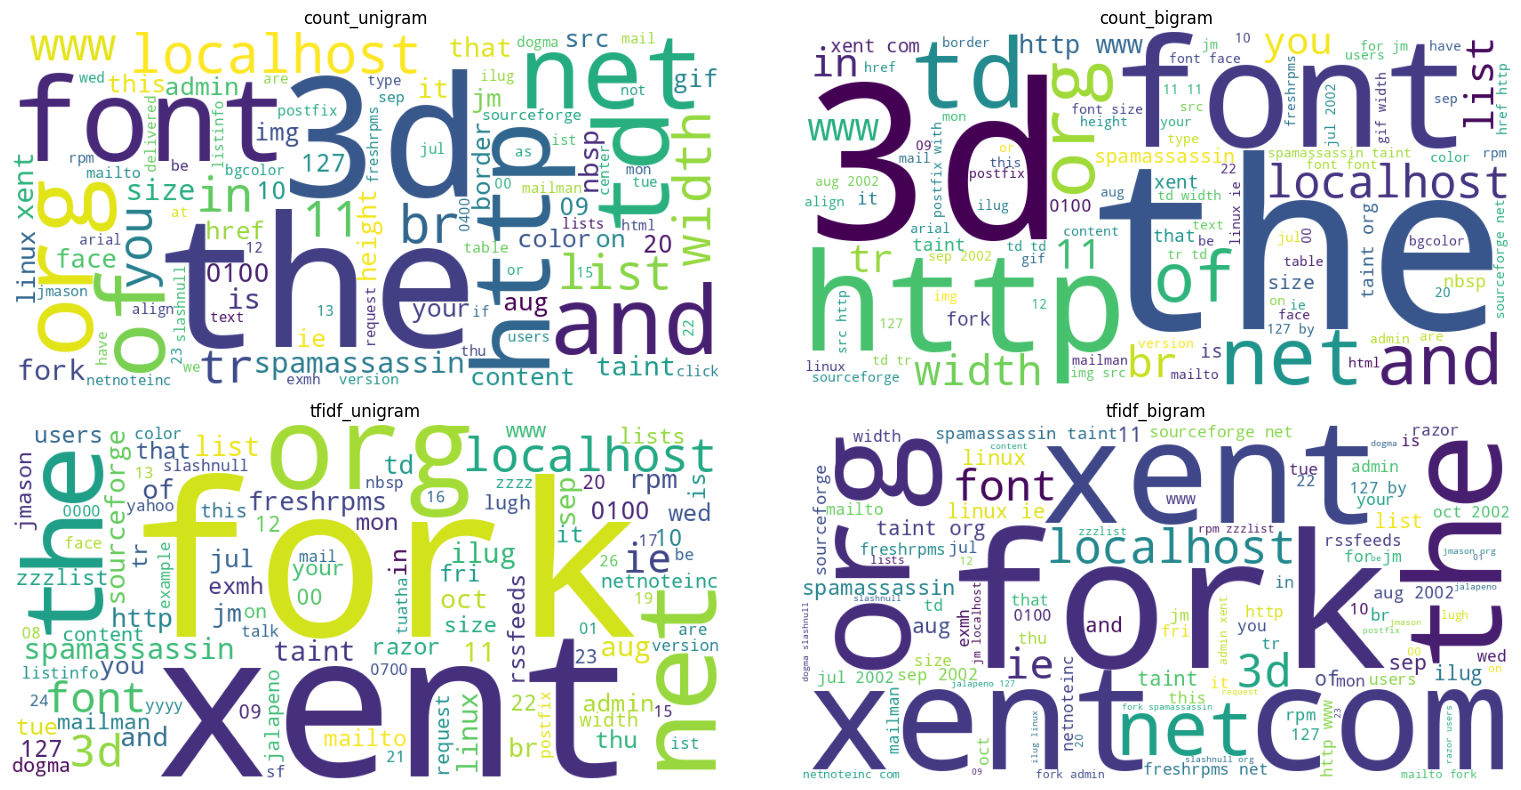
\includegraphics[width=0.95\linewidth]{imgs/00_preprocessing_word_cloud.png}
    \caption{Porównanie najczęstszych słów po wektoryzacji}
    \label{fig:enter-label}
\end{figure}

\subsection{Wyniki}
\begin{figure}[H]
    \centering
    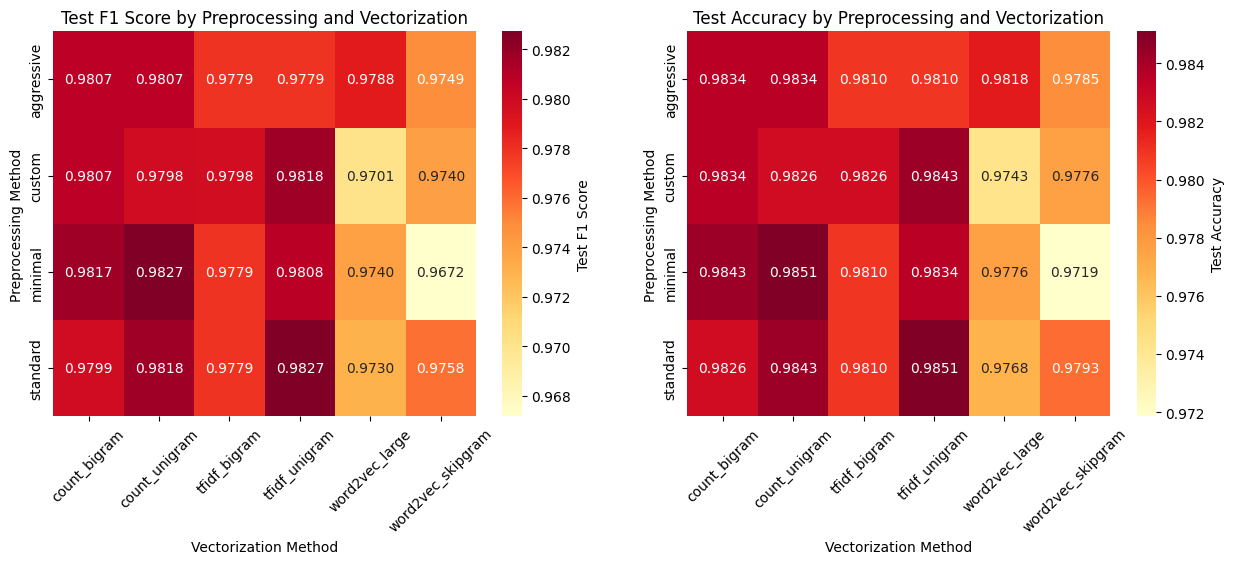
\includegraphics[width=1\linewidth]{imgs/01_preprocessing_vec_vs_preprocess.png}
    \caption{Zestawienie preprocessingu i wektoryzacji}
    \label{fig:enter-label}
\end{figure}

\begin{figure}[H]
    \centering
    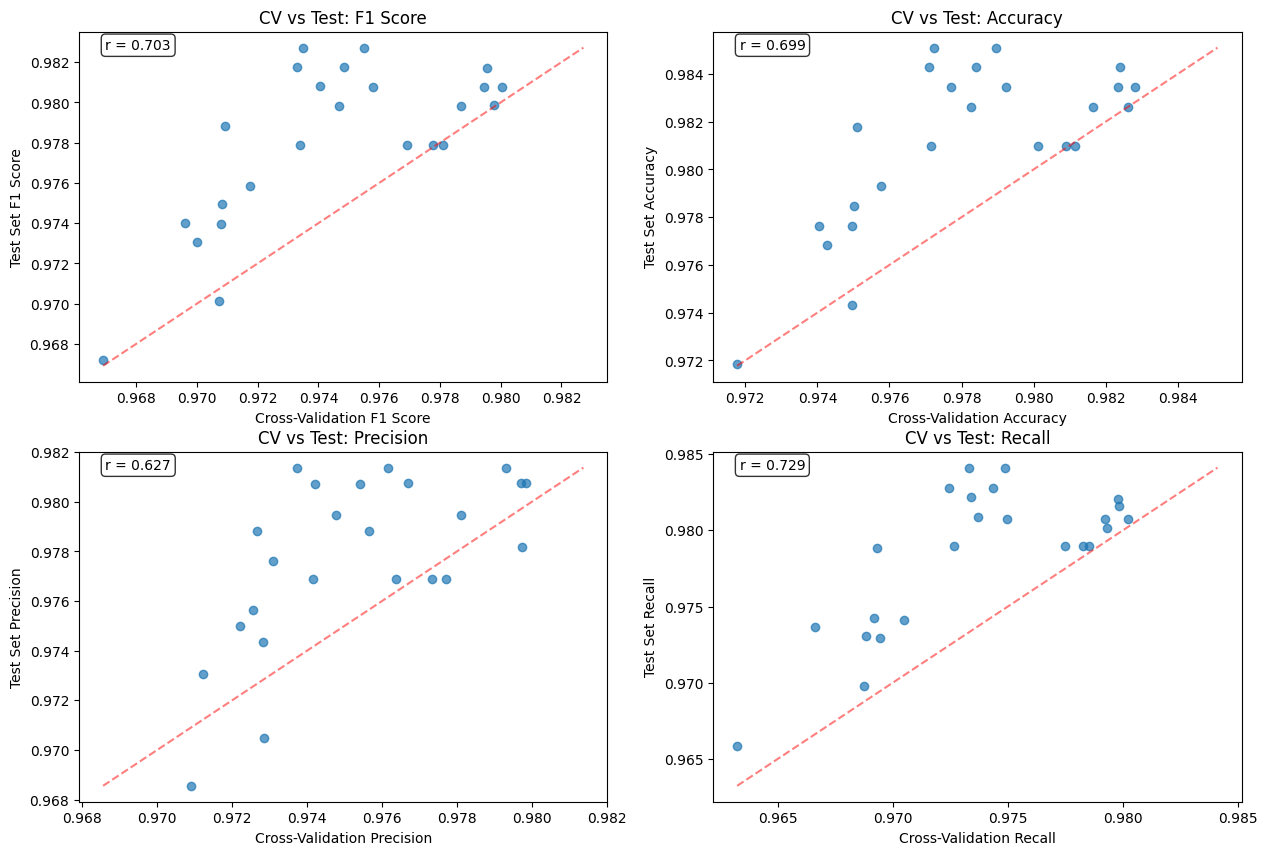
\includegraphics[width=0.8\linewidth]{imgs/02_preprocessing_cv_vs_test_comp.png}
    \caption{Porównanie wyników walidacji krzyżowej i zbioru testowego}
    \label{fig:enter-label}
\end{figure}

\begin{figure}[H]
    \centering
    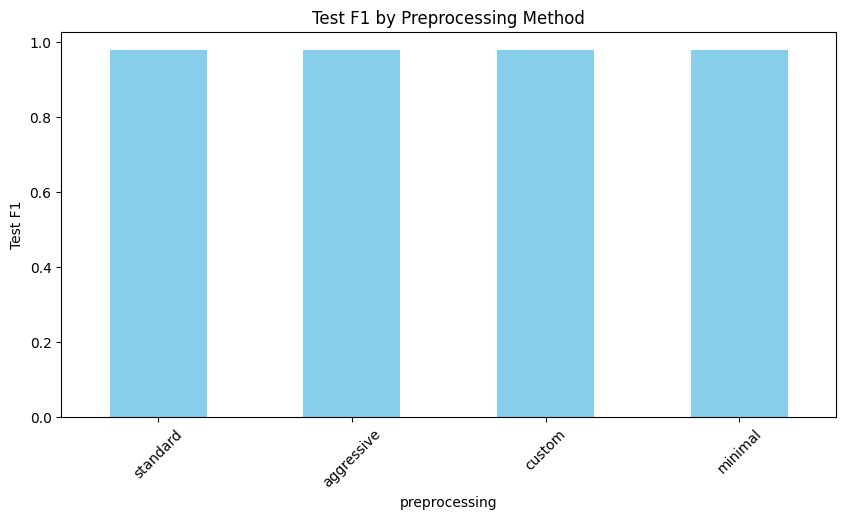
\includegraphics[width=0.7\linewidth]{imgs/03_preprocessing_prep_comp.png}
    \caption{Uśrednione wyniki ze względu na przetwarzanie}
    \label{fig:enter-label}
\end{figure}

\subsection{Wnioski}

Z przeprowadzonych eksperymentów wynika iż największy wpływ na wyniki ma rodzaj użytej reprezentacji. Rodzaj preprocessingu ma znikome znaczenie na finalną metrykę. Porównanie wyników walidacji krzyżowej i ze zbioru testowego potwierdza iż występuje konieczność wykonywania tych procedur, a także że rodzaj obróbki/reprezentacji może mieć dość znaczący wpływ na wyniki na produkcji - korelacja punktów jest dośc odległa od idealnej.

Najlepsze rezultaty uzyskały najprostsze metody: TF-IDF/BOW unigram z standardowym preprocessingiem(mała litera; brak interpunkcji/liczb/stop słów). Dość zaskakującym rezultatem są gorsze wyniki Word2Vec - pomimo standardowej długości treningu metoda okazała się najgorsza.

Stemming/agresywna obróbka pogarsza rezultaty z racji łączenia form, które w spamie mogą mieć silny sygnał.

\newpage

\section{Porównanie algorytmów}

W ramach serii eksperymentów porównane zostały algorytmy:
\begin{itemize}
    \item \textbf{MultinomialNB}
    \begin{itemize}
        \item \texttt{alpha}: wygładzanie Laplace; większe \texttt{alpha} może zmniejszyć ryzyko nadmiernego dopasowania
    \end{itemize}
    
    \item \textbf{SVM}
    \begin{itemize}
        \item \texttt{C}: współczynnik regularyzacji (szerokość marginesu)
        \item jądro liniowe; RBF -- nieliniowe granice
    \end{itemize}

    \item \textbf{Random Forest}
    \begin{itemize}
        \item \texttt{n\_estimators}: liczba drzew w lesie; lepsza stabilność i dokładność
        \item \texttt{max\_depth}: maksymalna głębokość drzewa; mniejsza głębokość zmniejsza przeuczenie
        \item \texttt{max\_features}: \% cech losowych przy podziale węzła
        \item \texttt{class\_weight}: wpływ czy balansować rozkład klas
    \end{itemize}

    \item \textbf{XGBoost}: zespół drzew budowany sekwencyjnie na podstawie wzmocnienia gradientowego różnicy predykcji i składników regularyzacji
    \begin{itemize}
        \item \texttt{max\_depth}: maksymalna głębokość drzewa
        \item \texttt{min\_child\_weight}: minimalna suma ważonych obserwacji w liściu
        \item \texttt{learning\_rate}: skalowanie wkładu nowego drzewa
        \item \texttt{subsample}: procent przykładów losowany do budowy drzewa
        \item \texttt{colsample\_bytree}: procent cech losowany do każdej struktury drzewa
    \end{itemize}
\end{itemize}

\subsection{Konfiguracja eksperymentów}

W ramach eksperymentów użyto preprocessingu: 
\texttt{\{'lowercase': True, 'remove\_punctuation': True, 'remove\_numbers': True, 'remove\_stopwords': True, 'stemming': False\}} 
oraz wektoryzacji TF-IDF bigram.

Dla każdego algorytmu przeprowadzono przegląd siatki hiperparametrów, a dla wyłonionych najlepszych parametrów wykonano trening, walidację krzyżową oraz ewaluację.

\begin{table}[h!]
\centering
\begin{tabular}{>{\bfseries}l l l}
\toprule
Model & Parameter & Values \\
\midrule
\multirow{1}{*}{MultinomialNB} 
    & alpha & [0.1, 0.5, 1.0, 2.0, 5.0] \\
\midrule
\multirow{1}{*}{SVM\_Linear} 
    & C & [0.1, 1.0, 10.0, 100.0] \\
\midrule
\multirow{2}{*}{SVM\_RBF} 
    & C & [0.1, 1.0, 10.0] \\
    & gamma & [\textquotesingle scale\textquotesingle, \textquotesingle auto\textquotesingle, 0.001, 0.01] \\
\midrule
\multirow{4}{*}{RandomForest} 
    & n\_estimators & [100, 300] \\
    & max\_depth & [None, 20] \\
    & max\_features & [\textquotesingle sqrt\textquotesingle] \\
    & class\_weight & [None, \textquotesingle balanced\textquotesingle] \\
\midrule
\multirow{5}{*}{XGBoost} 
    & max\_depth & [4, 6] \\
    & min\_child\_weight & [1, 4] \\
    & learning\_rate & [0.05, 0.1] \\
    & subsample & [0.85] \\
    & colsample\_bytree & [0.85] \\
\bottomrule
\end{tabular}
\caption{Parametry siatki dla poszczególnych modeli}
\end{table}


\begin{table}[h!]
\centering
\begin{tabular}{|l|p{10cm}|}
\hline
\textbf{Model} & \textbf{Najlepsze parametry} \\
\hline
MultinomialNB & \texttt{model\_\_alpha: 0.1} \\
\hline
SVM\_Linear & \texttt{model\_\_C: 100.0} \\
\hline
SVM\_RBF & \texttt{model\_\_C: 10.0, model\_\_gamma: 'scale'} \\
\hline
RandomForest & \texttt{model\_\_class\_weight: None, model\_\_max\_depth: None, model\_\_max\_features: 'sqrt', model\_\_n\_estimators: 300} \\
\hline
XGBoost & \texttt{model\_\_colsample\_bytree: 0.85, model\_\_learning\_rate: 0.1, model\_\_max\_depth: 6, model\_\_min\_child\_weight: 1, model\_\_subsample: 0.85} \\
\hline
\end{tabular}
\caption{Najlepsze parametry dla każdego modelu na podstawie eksperymentu}
\end{table}

\subsection{Wyniki}

\begin{figure}[H]
    \centering
    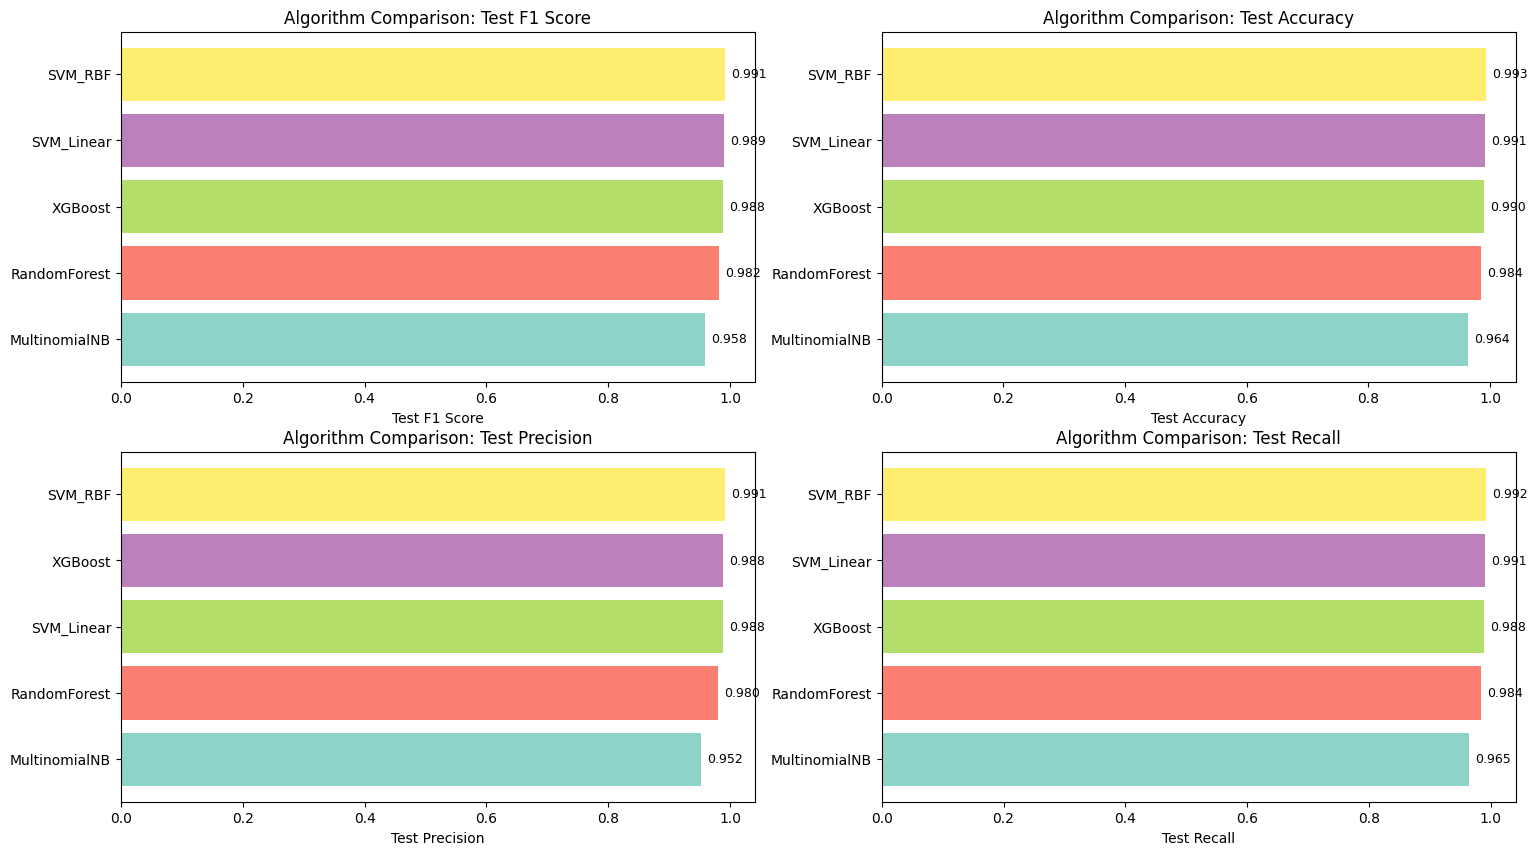
\includegraphics[width=1\linewidth]{imgs/04_algorithm_comparison.png}
    \caption{Porównanie wyników algorytmów}
    \label{fig:enter-label}
\end{figure}

\begin{figure}[H]
    \centering
    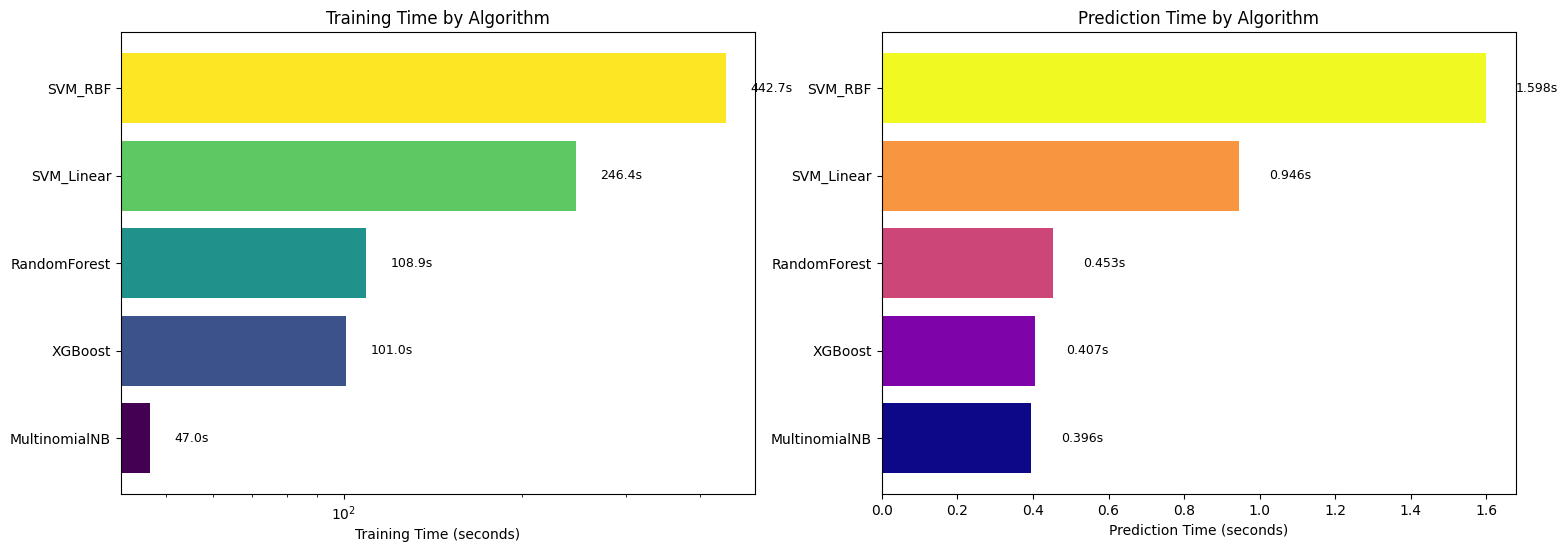
\includegraphics[width=1\linewidth]{imgs/05_algorithm_time.png}
    \caption{Porównanie czasów}
    \label{fig:enter-label}
\end{figure}

\begin{figure}[H]
    \centering
    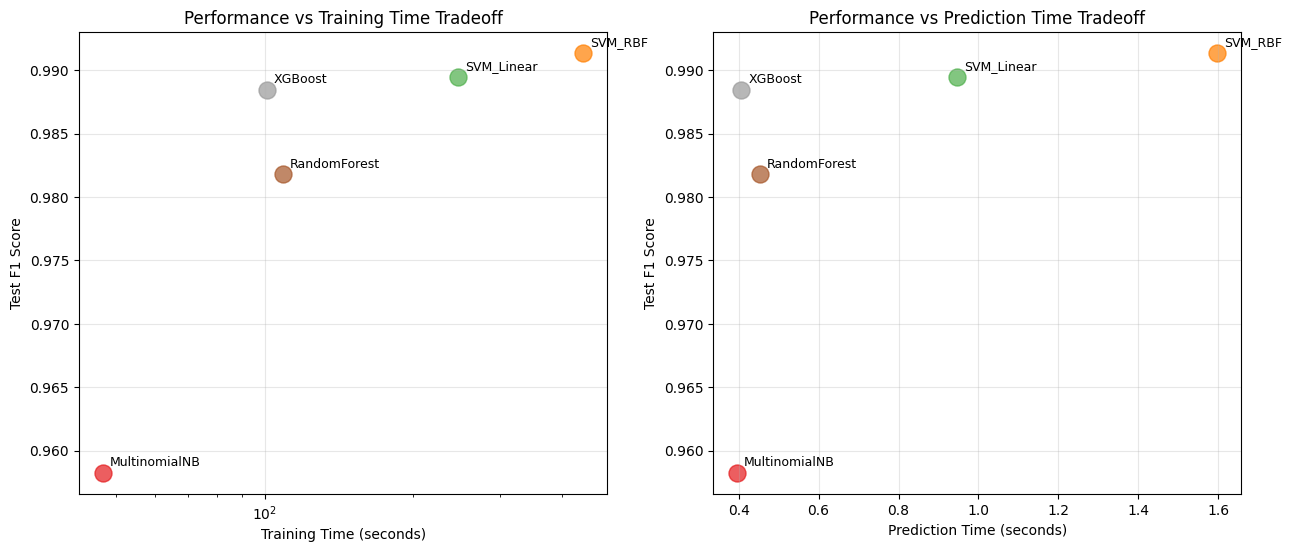
\includegraphics[width=1\linewidth]{imgs/06_algorithm_performance_vs_time.png}
    \caption{Zestawienie czasu wykonania i osiagów modelów}
    \label{fig:enter-label}
\end{figure}

\begin{figure}[H]
    \centering
    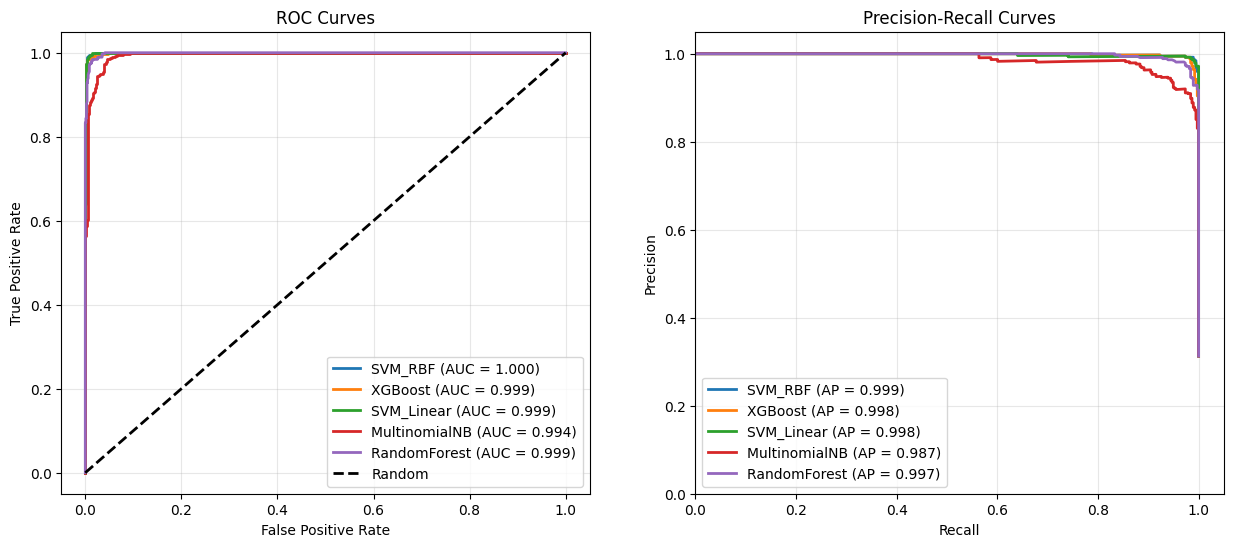
\includegraphics[width=1\linewidth]{imgs/07_algorithm_roc.png}
    \caption{Krzywe ROC i PR}
    \label{fig:enter-label}
\end{figure}

Wszystkie bardziej zaawansowane algorytmy osiągają F1 $>0.98$, jedynie Naiwny Bayes lekko odstaje od pozostałych. Prawdziwa jest również ta zależność dla czasu treningu: MultinomialNB uczy się 10x szybciej niż model o najlepszym F1. Z wykresu zestawiającego jakość do czasu treningu/inferencji wynika, iż najlepszymi modelami do tego zadania są XGBoost/SVM \_Linear, które mają najlepszy stosunek jakości do długości treningu.

W przypadku systemów krytycznych najlepszym rozwiązaniem okazałby się model SVM z nieliniowym jądrem, natomiast w prostszych systemach wystarczający mógłby być naiwny bayes/XGBoost.

Na podstawie krzywych ROC/PR można stwierdzić iż wszystkie modele poza naiwnym bayesem oferują bliską perfekcji separację, z czego wynika iż dalsza poprawa wymagałaby dalszej inżynierii cech danych.

\begin{figure}[H]
    \centering
    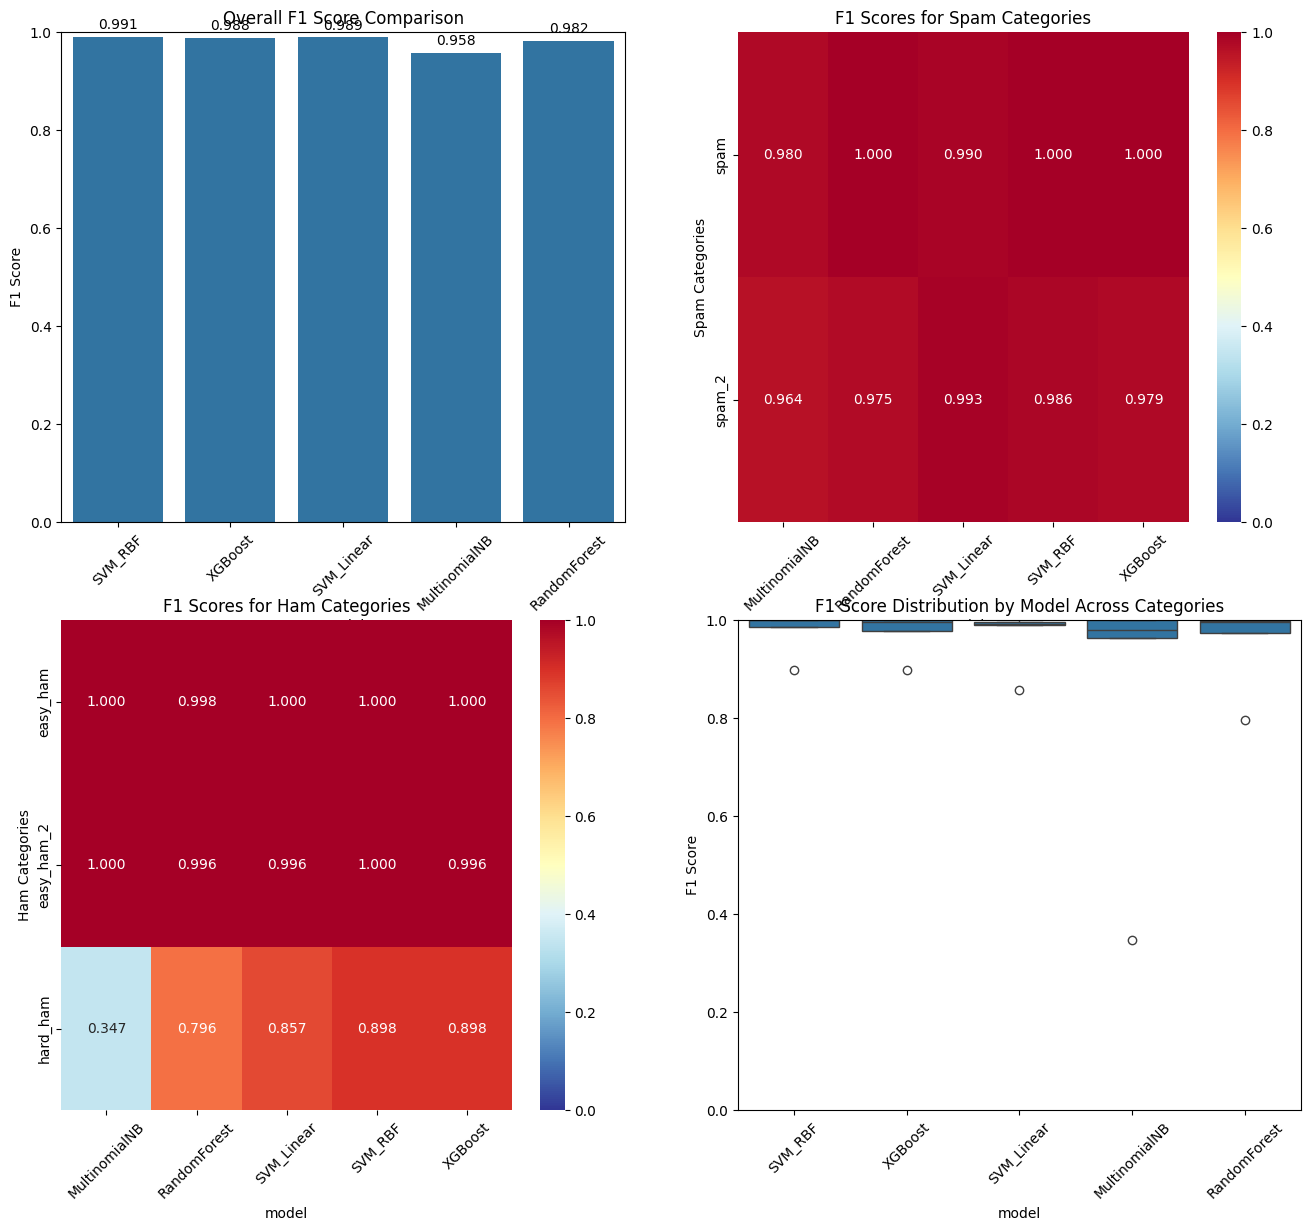
\includegraphics[width=1\linewidth]{imgs/08_algorithm_by_category.png}
    \caption{Wyniki modelu ze względu na podklasę spam/ham}
    \label{fig:enter-label}
\end{figure}

Kategoria trudnego hamu ujawnia faktyczne różnice w modelach - naiwny bayes radzi sobie znacząco gorzej niż inne modele - dodatkowo najlepszym algorytmem nadal pozostaje nieliniowy SVM.

\newpage

\section{Zastosowanie redukcji wymiarowości}

W ramach eksperymentu porównano wpływ różnych metod redukcji wymiarowości na jakość klasyfikacji mierzoną miarą F1 (na zbiorze testowym). Rozważone zostały następujące podejścia:

\begin{itemize}
    \item \textbf{baseline} — brak redukcji wymiarowości (pełny zbiór cech)
    
    \item \textbf{PCA (Principal Component Analysis)}:
    \begin{itemize}
        \item liczba komponentów: 50, 100, 200
    \end{itemize}
    
    \item \textbf{SVD (Singular Value Decomposition)}:
    \begin{itemize}
        \item liczba komponentów: 50, 100, 200
    \end{itemize}
    
    \item \textbf{SelectKBest (z testem statystycznym)} - ANOVA F(sprawdza średnią wartość cechy F pomiędzy klasami pozwalając na eliminację):
    \begin{itemize}
        \item liczba wybranych cech: 50, 100, 200, 500
    \end{itemize}
\end{itemize}

\subsection{Konfiguracja eksperymentów}

W ramach eksperymentów modelem bazowym był liniowy SVM(u którego ilość wymiarów ma znaczenie na czas treningu), dane były obrobione wariantem \texttt{standard}.

\subsection{Wyniki}

\begin{figure}[H]
    \centering
    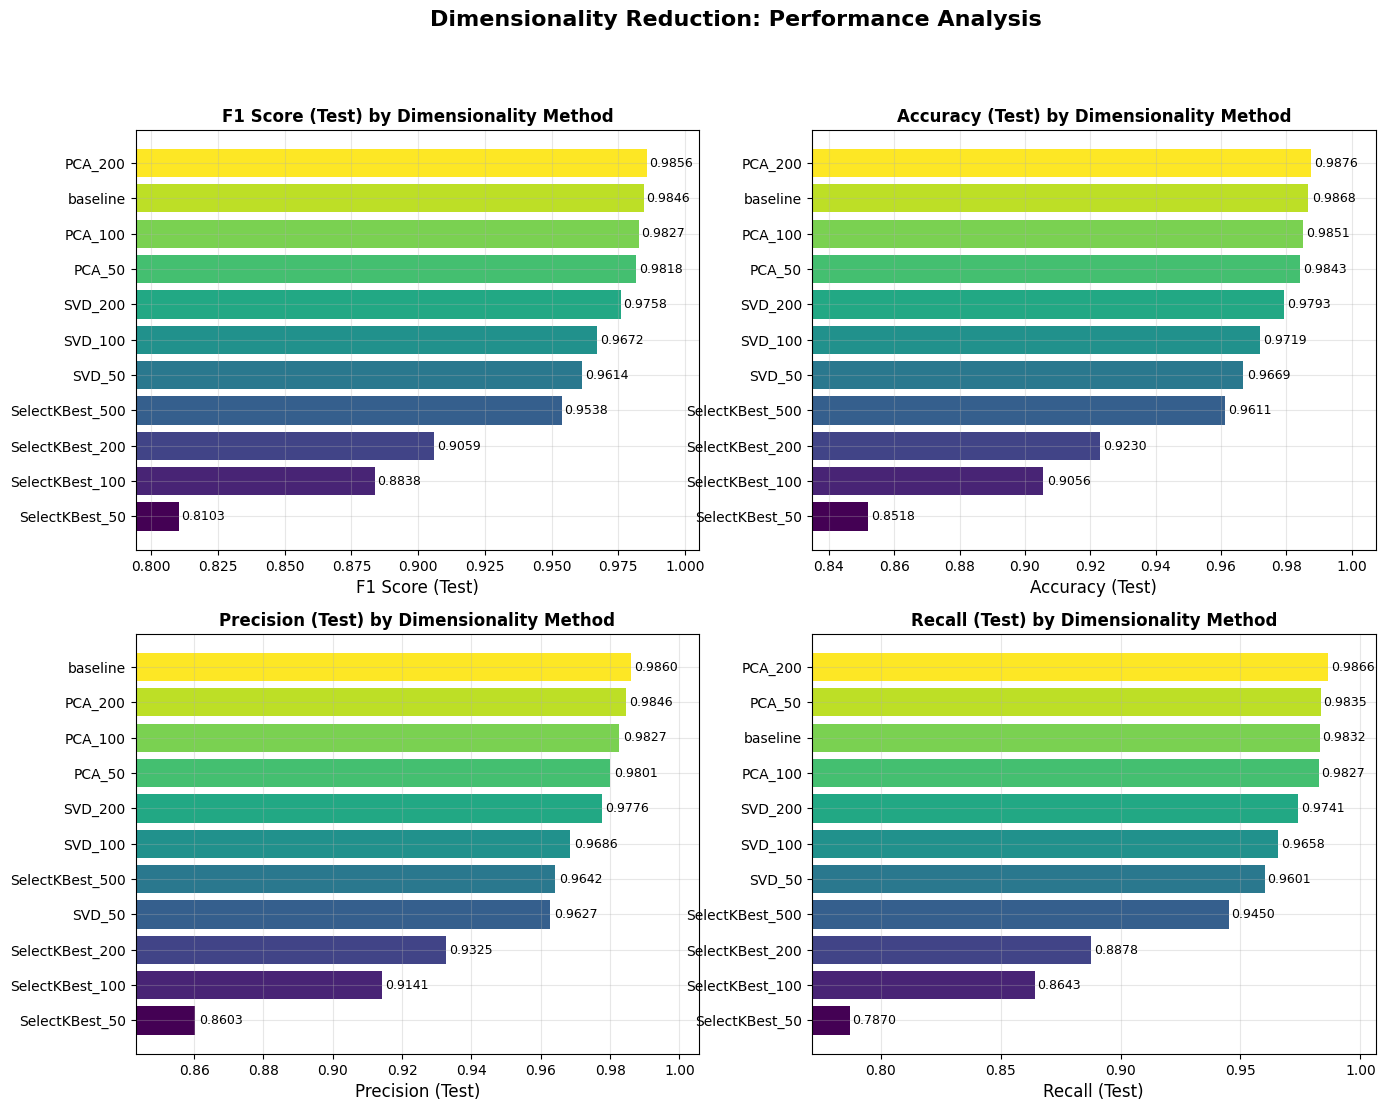
\includegraphics[width=1\linewidth]{imgs/09_reduction_metrics.png}
    \caption{Zestawienie metryk}
    \label{fig:enter-label}
\end{figure}

\begin{figure}[H]
    \centering
    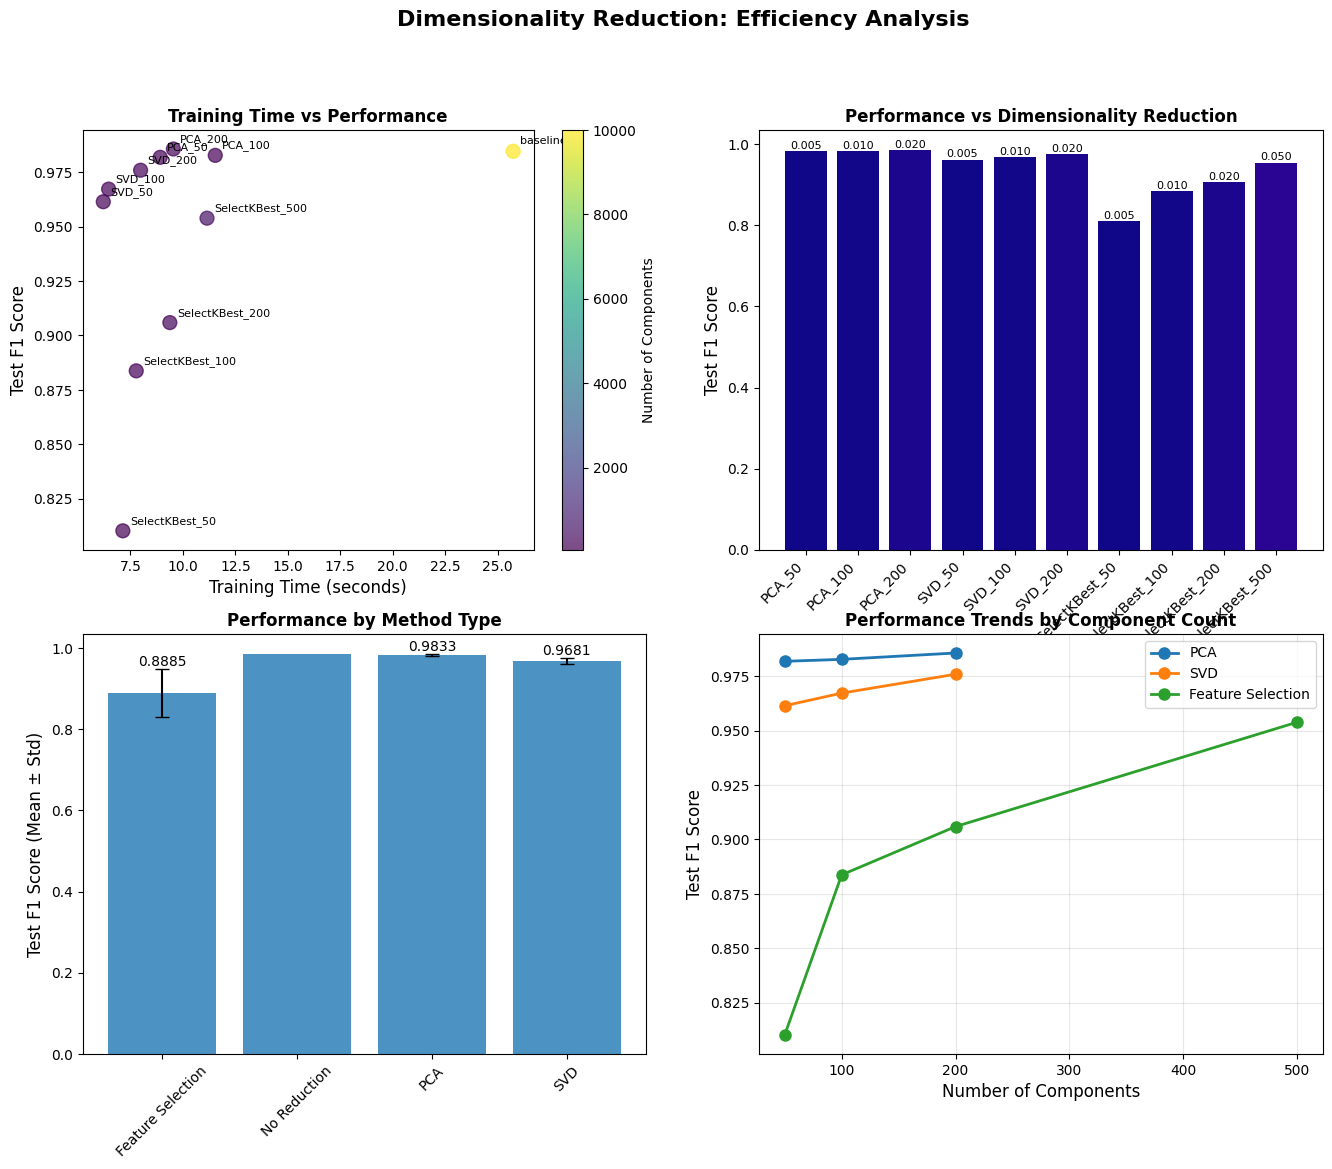
\includegraphics[width=1\linewidth]{imgs/10_reduction_time.png}
    \caption{Wpływ redukcji na czas uczenia i jakość}
    \label{fig:enter-label}
\end{figure}

\begin{figure}[H]
    \centering
    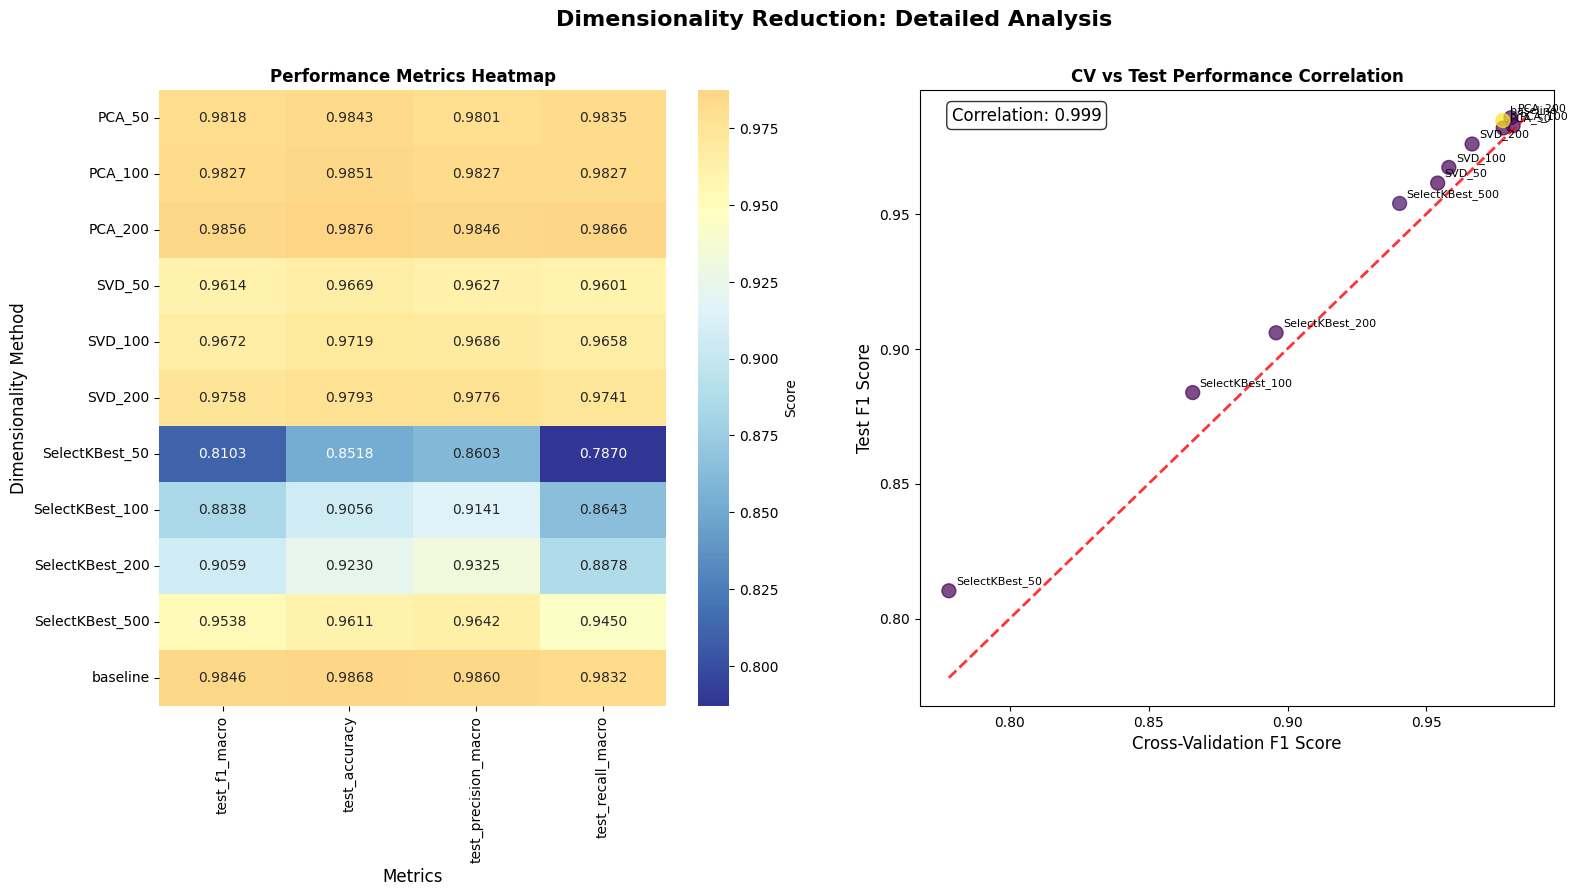
\includegraphics[width=1\linewidth]{imgs/11_reduction_heatmap.png}
    \caption{Heatmapa i porównanie z walidacją krzyżową}
    \label{fig:enter-label}
\end{figure}

Wariant PCA\_200 osiąga jakość podobną do wariantu bazowego przy ponad 2-krotnym zmniejszeniu czasu treningu. Warianty SVD są szybsze niż PCA, jednakże zawsze lekko gorsze - SVD\_50 osiąga akceptowalną jakość przy znacznym zmniejszeniu zapotrzebowania pamięci. Pomysł z odrzucaniem słów przy pomocy testu statystycznego okazał się nie trafiony i osiąga zawsze odstające wyniki.

\newpage

\section{Podsumowanie}

W trzech blokach eksperymentów zaprezentowano pełną ścieżkę projektowania skutecznego filtra spamu:

\begin{itemize}
    \item \textbf{Obróbka i reprezentacja:}
    \begin{itemize}
        \item Największy wpływ na metryki miała sama reprezentacja tekstu.
        \item Klasyczne metody takie jak \textbf{TF-IDF} lub \textbf{Bag-of-Words (BoW)} w wariancie unigram przewyższały zaawansowane embeddingi \texttt{Word2Vec}.
        \item Agresywne czyszczenie danych (np. stemming, usuwanie liczb) nie przynosiło korzyści, a wręcz zubażało sygnał.
        \item Najlepsze rezultaty osiągał prosty pipeline:
        \begin{itemize}
            \item konwersja do małych liter (\texttt{lowercase}),
            \item usunięcie interpunkcji, liczb oraz słów nieinformacyjnych (\texttt{stop-words}),
            \item wektoryzacja \textbf{TF-IDF unigram}.
        \end{itemize}
    \end{itemize}
    
    \item \textbf{Dobór algorytmu:}
    \begin{itemize}
        \item Wszystkie „cięższe” modele, z wyjątkiem Naiwnego Bayesa, osiągnęły F1 większe niż 0{,}98.
        \item \textbf{XGBoost} oraz \textbf{SVM z jądrem liniowym} oferowały najlepszy stosunek jakości do czasu uczenia i predykcji.
        \item \textbf{SVM z jądrem RBF} osiągnął najwyższy wynik F1 ≈ 0{,}991, ale wymagał około czterokrotnie dłuższego czasu treningu.
        \item \textbf{MultinomialNB} był dziesięciokrotnie szybszy, lecz generował więcej fałszywych alarmów w kategorii „hard ham”.
    \end{itemize}

    \item \textbf{Redukcja wymiarowości:}
    \begin{itemize}
        \item \textbf{PCA} z 200 składowymi utrzymywała (a czasami poprawiała) dokładność modelu bazowego, skracając czas treningu ponad dwukrotnie.
        \item \textbf{SVD} było nieco słabsze jakościowo, ale miało najniższe wymagania pamięciowe.
        \item Wybór cech metodą \texttt{SelectKBest} (ANOVA F-score) był niewystarczający -- przy \texttt{k ≤ 200} wartość F1 spadała nawet o 17 p.p. względem wariantu bazowego.
    \end{itemize}
\end{itemize}

\subsection*{Wnioski kluczowe}

\begin{itemize}
    \item \ TF-IDF unigram wraz z umiarkowanym preprocessingiem zapewnia najwyższy i najbardziej stabilny wynik F1 przy minimalnym nakładzie obliczeniowym.
    
    \item \textbf{Model zależy od budżetu:} 
    \begin{itemize}
        \item dla zastosowań produkcyjnych o dużej skali zalecany jest \textbf{XGBoost} lub \textbf{SVM Linear},
        \item w systemach krytycznych, gdzie liczy się ostatnie 0{,}2 p.p. F1, warto wybrać \textbf{SVM RBF},
        \item na urządzeniach o małej mocy można zaakceptować \textbf{MultinomialNB}.
    \end{itemize}

    \item PCA z 100–200 komponentami zachowuje wysoką precyzję, a jednocześnie znacząco skraca czas treningu i zmniejsza rozmiar modelu, co ułatwia wdrożenie w środowiskach z ograniczoną pamięcią.
\end{itemize}

\end{document}